\subsection{Discrete Event Driven Decision Points}
\label{sec:discerete_event}
So far, one of the defining characteristics of the considered scheduling problem—namely stochastic and heterogeneous job arrivals—has been introduced. Jobs enter the system dynamically at unpredictable times, leading to a production environment that continuously evolves over time. As new jobs arrive, ongoing operations are completed, resources are released, and other jobs simultaneously reach points at which scheduling decisions are required. Consequently, decision-relevant moments in the system are no longer aligned with fixed time steps but are instead determined by events occurring in real time. This necessitates an adaptation of the decision-making mechanism to remain consistent with the dynamic nature of the system.

At this point, it is useful to recall the decision point implementation adopted in the standard MASA-QMIX baseline. In that formulation, decision making is organised around a discrete, time-driven structure in which all agents act synchronously at globally unified decision instants. Decision times are indexed by $k$ and progress deterministically starting from an initial decision time $t_0$, such that the $k$-th decision is taken at time $t_k$, while the subsequent decision is scheduled at $t_{k+1}$ after a constant decision interval. This fixed interval, denoted by $\Delta t$ in the baseline formulation (cf. Eq.~\eqref{eq:decision_time_grid}), defines the temporal resolution of the decision-making process and remains unchanged throughout the episode. As a consequence, execution between two consecutive decision instants $t_k$ and $t_{k+1}$ is treated as continuous but remains unobservable to the decision mechanism, and all state updates and scheduling reactions are incorporated only when the next decision time is reached. This design enforces a globally synchronised decision structure, where each decision point corresponds to a snapshot of the system state taken at multiples of the fixed interval $\Delta t$.

While this time-driven design is well suited to the static and closed assumptions of the standard MASA-QMIX setting, its limitations become apparent when applied to a dynamic environment with stochastic job arrivals and asynchronous operation completions. To illustrate this mismatch, we now examine how the baseline decision-time structure behaves when applied to the scheduling problem considered in this work.

Assume a unit decision interval and consider a decision taken at time $t_1 = 1$, with the next decision scheduled at $t_2 = 2$. Within this interval, a sequence of execution events occurs at continuous times,
\[
\mathcal{E}_{\text{ex}} = \{ e_1, e_2, e_3, e_4, e_5 \},
\qquad
\text{with}
\qquad
t_{e_1} = 1.10,\;
t_{e_2} = 1.25,\;
t_{e_3} = 1.51,\;
t_{e_4} = 1.74,\;
t_{e_5} = 1.89.
\]
The events in $\mathcal{E}_{\text{ex}}$ occur in chronological order within the decision interval $(1,2)$. Specifically, $e_1$, $e_3$, and $e_5$ correspond to job arrival events, while $e_2$ and $e_4$ represent operation completion events. Despite occurring at distinct continuous times, all events in $\mathcal{E}_{\text{ex}}$ are first observed by the decision-making mechanism only at the next unified decision point $t_2 = 2$ under the standard MASA-QMIX execution logic.

Formally, the baseline abstraction induces the mapping
\[
t_{e_r} \mapsto t_2, \qquad \forall e_r \in \mathcal{E}_{\text{ex}},
\]
thereby collapsing multiple distinct execution events into a single decision instant.

The delay introduced by this abstraction can be quantified by defining a temporal abstraction error for each event. For an event $e_r$ occurring at time $t_{e_r} = t_1 + \delta_r$ with $\delta_r \in (0,1)$, the abstraction error is given by
\[
\varepsilon_r = t_2 - t_{e_r} = \Delta t - \delta_r.
\]
For the above event sequence, this yields:
\[
\varepsilon_1 = 0.90, \quad
\varepsilon_2 = 0.75, \quad
\varepsilon_3 = 0.49, \quad
\varepsilon_4 = 0.26, \quad
\varepsilon_5 = 0.11.
\]
Thus, within a single decision interval, multiple events experience different delays, even though all are treated as if they occurred at the same time $t = 2$. This destroys the temporal ordering of events and limits the system's ability to react in a time-accurate manner. This temporal collapse is illustrated in Figure~\ref{fig:temporal_abstraction}, which visualizes the distortion introduced by the fixed decision grid.

\begin{figure}[htbp]
\centering
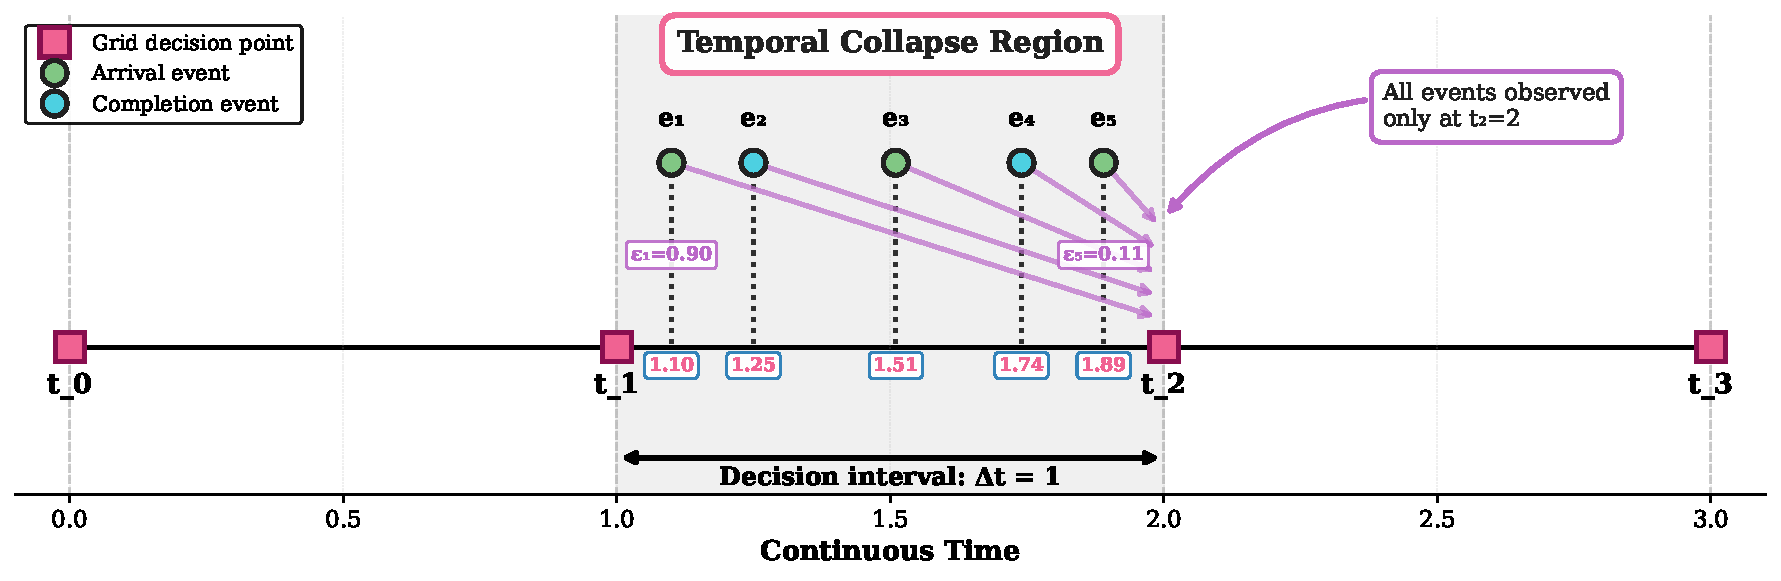
\includegraphics[width=0.9\textwidth]{docs/temporal_abstraction.pdf}
\caption{Temporal abstraction error under fixed-interval decision making. Events $e_1, \ldots, e_5$ occurring at distinct continuous times within the interval $(t_1, t_2)$ are all collapsed to the next grid decision point $t_2$, introducing delays $\varepsilon_r = t_2 - t_{e_r}$. This temporal collapse destroys event ordering and causes systematic bias in scheduling decisions.}
\label{fig:temporal_abstraction}
\end{figure}

The temporal abstraction is particularly critical for job arrivals. For example, the true inter-arrival time between the first and last arriving jobs is
\[
\Delta t_{\text{arr,true}} = 1.89 - 1.10 = 0.79,
\]
whereas under the baseline abstraction both arrivals are first observed at $t_2 = 2$, resulting in a perceived inter-arrival time of
\[
\Delta t_{\text{arr,grid}} = 0.
\]
Consequently, arrival dynamics and congestion evolution cannot be inferred consistently, as distinct arrival times are temporally collapsed.

A similar distortion arises for operation completions. If a job completes an operation at $t_{e_2} = 1.25$ and becomes immediately ready to proceed, the baseline design delays the next decision opportunity until $t_2 = 2$, introducing an artificial waiting time of
\[
w_{\text{artificial}} = t_2 - t_{e_2} = 0.75.
\]
This waiting time is not caused by resource contention but solely by the fixed decision-time discretisation, leading to systematically biased waiting-time and flow-time measurements. Such distortions may constitute up to 75\% of the actual processing time in typical manufacturing operations, systematically corrupting reward signals and biasing policy learning toward suboptimal scheduling decisions.

These observations demonstrate that the fixed unified decision-time design of the standard MASA-QMIX baseline is incompatible with dynamic scheduling environments characterised by stochastic job arrivals and asynchronous operation completions. \textbf{These limitations motivate the adoption of an event-driven decision formulation, which requires explicit discrete-event simulation capabilities.}

\paragraph{Why Discrete-Event Simulation is Required for Event-Driven Decision Making}

In the considered scheduling problem, system-relevant state changes occur only at execution events, such as job arrivals and operation completions. Between two such events, the system state remains unchanged. Formally, letting
\begin{equation}
\mathcal{E} = \{ e_1, e_2, \ldots \}
\label{eq:event_set}
\end{equation}
denote the set of execution events with occurrence times $t_e \in \mathbb{R}_{\ge 0}$, the system state satisfies
\begin{equation}
\mathcal{S}(t_e^+) \neq \mathcal{S}(t_e^-),
\label{eq:state_jump_at_event}
\end{equation}
while remaining constant between events,
\begin{equation}
\mathcal{S}(t) = \mathcal{S}(t_e), 
\qquad \forall t \in (t_e, t_{e+1}).
\label{eq:state_constant_between_events}
\end{equation}

This property implies \emph{temporal sparsity}: meaningful state transitions occur only at event times. A time-stepped reinforcement learning formulation, which advances the environment at fixed intervals $\Delta t$, therefore performs unnecessary state updates. Over an episode of length $T$, such a formulation requires
\begin{equation}
\mathcal{O}\!\left(\frac{T}{\Delta t}\right)
\label{eq:time_step_complexity}
\end{equation}
state transitions, even though only $N_{\text{events}}$ execution events occur, with
\begin{equation}
N_{\text{events}} \ll \frac{T}{\Delta t}.
\label{eq:event_vs_timestep}
\end{equation}
As a result, time-stepped formulations either waste computation for small $\Delta t$ or risk missing execution events for larger $\Delta t$.

More importantly, reinforcement learning alone does not maintain a notion of continuous physical time. State transitions are indexed only by a step counter $k$,
\begin{equation}
\mathcal{S}_k \rightarrow \mathcal{S}_{k+1},
\label{eq:rl_step_transition}
\end{equation}
and any execution events occurring between two steps are indistinguishable. In the standard MASA-QMIX baseline, this limitation is masked by manually associating each learning step with a fixed decision interval. However, this abstraction breaks down in dynamic environments with stochastic job arrivals and asynchronous operation completions, where execution events occur at irregular time instants.

Furthermore, realistic manufacturing systems involve explicit resource contention, where multiple jobs may compete for the same machine or operator. Correctly handling such contention requires synchronisation mechanisms to ensure mutual exclusion and blocking behaviour, which are not natively supported by reinforcement learning frameworks operating on abstract state transitions. These mechanisms are, however, inherently provided by \textbf{\emph{discrete-event simulation}} through resource queuing and blocking semantics.

To address these limitations, the reinforcement learning environment is integrated with a \textbf{\emph{discrete-event simulation}} framework. In this work, \textbf{\emph{SimPy}} is used to explicitly advance continuous time and execute events in chronological order, with deterministic priority-based scheduling for simultaneous events, ensuring reproducibility. The simulation layer governs physical time through the event sequence $\{t_e\}$, while reinforcement learning operates over discrete decision epochs aligned with these events.

Under this integration, decision making becomes event-driven: each decision point is triggered by an execution event,
\begin{equation}
e \;\Rightarrow\; \text{decision epoch},
\label{eq:decision_epoch_event}
\end{equation}
and the corresponding decision time is given by
\begin{equation}
t_{\text{decision}} = t_e.
\label{eq:decision_time_event}
\end{equation}
The elapsed time between consecutive decision epochs is therefore non-uniform and determined by the system dynamics as
\begin{equation}
\Delta t_e = t_{e+1} - t_e.
\label{eq:delta_te}
\end{equation}

This formulation ensures that no execution event is missed, causal ordering is preserved, and state transitions are evaluated at their true occurrence times. Consequently, \textbf{\emph{discrete-event simulation}} is not an implementation detail, but a structural requirement for accurate and efficient event-driven decision making in stochastic job shop scheduling.
